\renewcommand{\stagefigureprefix}{3}\setcounter{figure}{0}
\reporttitle{第三阶段：协同仿真与性能评估}

\section{从功能验证到工程评价}
自定义指令需要在程序中产生正确结果，也需要与处理器的异常、状态和调度机制配合。本阶段使用独立NEMU参考模型和全核DiffTest核对架构行为，再以等价RVV程序比较完整测量窗口的周期。另外给出软件接入方式，以及综合面积和静态时序结果，用于评估这项设计的收益与成本。主要结果是：RTL与NEMU参考模型在全部功能用例上协同仿真一致；相对等价的RVV程序，独立批量和依赖链场景分别加速3.07倍和2.93倍，单次点积加速1.20倍；独立批量的收益主要来自两槽流水，它比上一版单笔在途设计少用39\%的周期；8×32 GEMV函数调用快1.095倍；VDot功能单元的面积约占所在执行单元的6.0\%，在4\,ns约束下所有路径都满足setup要求。

本阶段的评估对象是最终提交的稳定版，即八项点积、两槽流水的实现（下文称“受测版本”），依次给出微基准、C8软件调用和完整前向计算的结果。VDot功能单元下文简称FU；它所在的向量执行单元VFEX4与整数除法、浮点除法/开方单元共享派发和写回，下文称为父级。第\ref{sec:3-cost}节还在相同综合条件下比较了SP1方案（把点积运算从两拍缩短为一拍），并附一组双工艺库参考数据。比较之后，最终提交仍采用稳定版，SP1作为优化探索保留。每组实验都注明了所用版本、输入和测量范围。

图\ref{fig:S3-01}给出本阶段的协同仿真框架。同一AM镜像与共同启动flash分别加载到香山DUT和固定NEMU参考端；DUT按架构提交推进参考模型，两端状态送入DiffTest，比较完整128位向量结果、约定的向量CSR和异常状态。运行配置冻结为单核、VLEN128和128MB内存，源码、二进制、配置、原始日志和真实退出码一并归档。两端的点积计算方式不同，参考端的具体处理见下节。

\reportfigure{S3-01}{RTL与独立参考模型的协同仿真}{9cm}{共同AM程序与启动flash驱动固定香山DUT和独立NEMU参考端，按架构提交推进并比较完整128位向量结果、约定的CSR与异常状态。两端内部求值组织不同，具体语义见下节；运行身份与原始输出分别归档。}{固定八项点积受测组合的DiffTest框架，图中版本仅适用于所示冻结组合。}

\section{NEMU参考语义与处理器接入}
RTL通过并行乘法、归约网络和流水状态执行点积；NEMU参考模型则从指令字、源寄存器和向量配置出发，顺序计算八项有符号乘积之和。两者的内部实现方式不同，因此可以相互核对。

参考端首先匹配custom-0编码并检查合法配置，随后快照读取两个源寄存器，计算点积并构造完整128位目的值：低32位为整数结果，高96位为零。快照读取使源、目的寄存器重合时仍使用本条指令执行前的数据。合法运算保留约定的向量状态；非法配置进入异常处理。

受测版本使用基于NEMU固定版本的vdot补丁及配套平台适配。适配使NEMU的xTVAL行为与该香山版本一致，异常码、陷阱PC、xTVAL和目的寄存器状态都在比较范围内；特权相关测试在M模式下完成。正常参考库与用于负控的故障注入库分别构建，各自记录来源和SHA-256。

图\ref{fig:S3-02}展示参考端的处理流程。参考端先精确匹配custom-0编码，未匹配的指令交给其他译码；再检查向量状态是否合法，即VS已启用、vtype合法、vl=8且vstart=0，非法时产生cause=2的非法指令异常且不写vd；合法时先快照两源的低64位，执行8项有符号点积，再完整写回128位结果，并在成功后将VS置脏。

\reportfigure{S3-02}{参考模型的译码、状态检查与完整写回}{9cm}{参考端先精确匹配编码并检查向量状态，再快照两源低64位、执行8项有符号点积并完整写回128位结果。非法状态产生异常且不写目的；合法执行后更新VS状态，xTVAL遵循固定平台适配规则。}{NEMU补丁说明及冻结参考模型的执行流程示意。}

\section{差分检验与错误检出}\label{sec:3-diff}
基础功能矩阵覆盖正数、负数、边界值、寄存器别名和非法向量配置。在受测版本上，全核矩阵包含117个不同用例，按矩阵分片共执行124次；数值正确性由算术RTL的10022项测试覆盖，握手控制由真实父级测试覆盖。最终验收时汇总了13项已有的全核记录和1项新增的控制诊断运行，并重新解析了它们的原始输出。

为了检验完整128位比较是否有效，负控在参考端的vdot结果中翻转bit100。差分器检测到目的寄存器高半区不一致并按预期终止；恢复正常参考模型后，同一程序完成15项检查并到达GOOD TRAP。图\ref{fig:S3-03}给出了这两个互补结果：前者检验错误检出能力，后者检验正常执行路径。负控日志中可见\texttt{v10\_high different}、\texttt{ABORT}和退出码1，差异出现在PC \texttt{0x80001bdc}；日志里的\texttt{right}和\texttt{wrong}只是比较器两侧的名称，本例的错误注入在参考端。正常日志的退出码为0。两段日志分别来自干净环境复现中的\texttt{negative-vdot}与\texttt{functional-0}运行。

% Original user screenshots; no cropping, redraw, or altered log content.
\begin{center}\begin{minipage}{\linewidth}\centering
\textbf{（a）参考端注错：检测到高位差异并中止}\par\smallskip
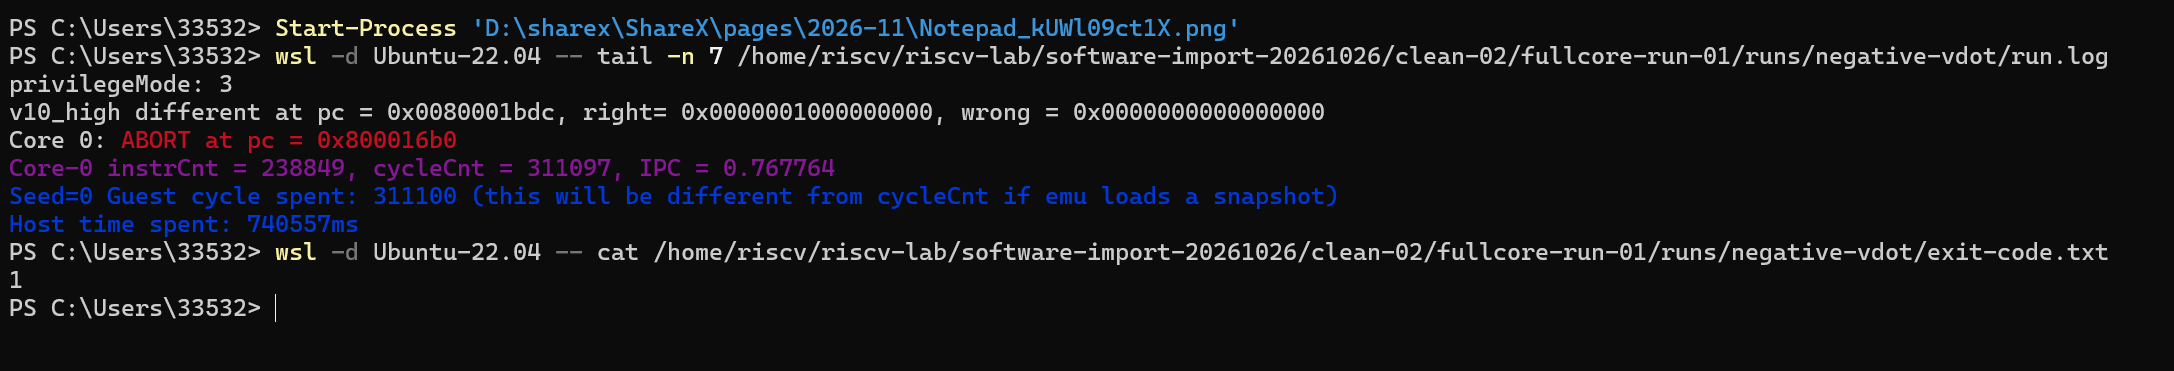
\includegraphics[width=\linewidth]{figures/source-screenshots/S3-03-01-bit100-rejection.png}
\par\medskip
\textbf{（b）正常参考模型：15项通过并正常退出}\par\smallskip
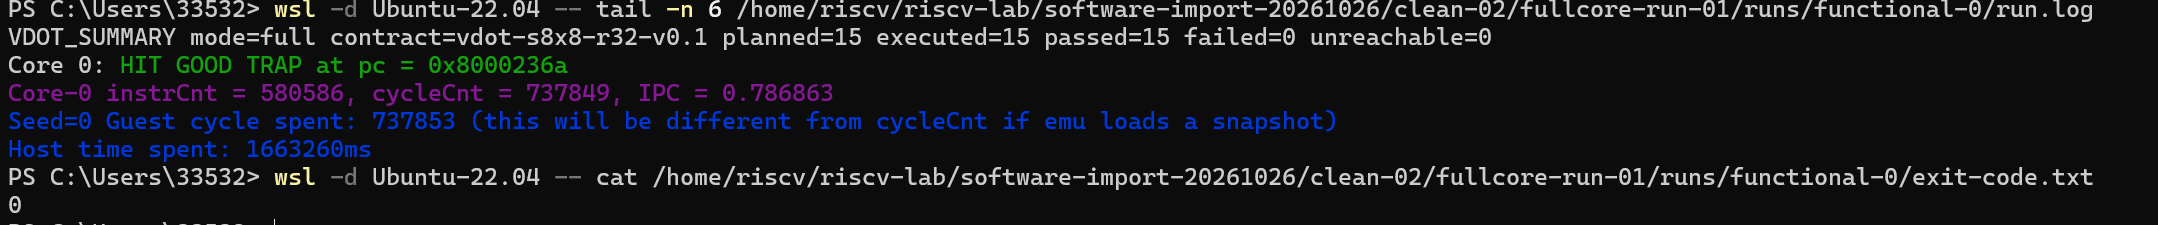
\includegraphics[width=\linewidth]{figures/source-screenshots/S3-03-02-normal-recovery.png}
\captionof{figure}{bit100拒错与正常参考模型恢复验证的原始日志截图}\label{fig:S3-03}
\raggedright\footnotesize
\textbf{注：}上图显示\texttt{v10\_high different}、\texttt{ABORT}及退出码1；差异PC为\texttt{0x80001bdc}，ABORT报告PC为\texttt{0x800016b0}，两者分别保留。参考端故意注错时，\texttt{right/wrong}为比较器两侧标签，不据此判定RTL本身有错。下图显示\texttt{planned=15 executed=15 passed=15 failed=0 unreachable=0}、\texttt{HIT GOOD TRAP}及退出码0。\par
\textbf{来源与范围：}用户提供的历史日志回读截图，来源为\seqsplit{/home/riscv/riscv-lab/software-import-20261026/clean-02/fullcore-run-01/runs/}下\texttt{negative-vdot}与\texttt{functional-0}目录的\texttt{run.log}和\texttt{exit-code.txt}。本次仅补入截图，未重新执行仿真；截图未展示机器字及完整128位结果，相关身份以原始运行记录为准。\par
\end{minipage}\end{center}

\section{vdot全核波形与事务核对}
2026年11月5日补充一次真实全核波形捕获。复用稳定0f对应clean-02封存生成RTL，1681项生成输入与原清单一致，在独立目录编译启用FST的新EMU，运行原functional-2镜像与正常NEMU。DiffTest开启，程序最终GOOD TRAP、真实退出码0。本次增加波形证据，不新增性能、面积或STA结论，也不改写原R5组合验收范围。\par

\subsection{输入、结果与事务身份}
两源均为\seqsplit{0xa5a5a5a5a5a5a5a50807060504030201}，低八个signed int8元素为1至8。数学预期为$1^2+2^2+\cdots+8^2=204$；实际128位响应为\seqsplit{0x000000000000000000000000000000cc}，高96位清零。源高64位A5哨兵不参与计算。\par
{\small\begin{longtable}{p{.24\linewidth}p{.68\linewidth}}\toprule
字段 & 核对值\\\midrule
事务身份 & ROB0:39；物理目的103（十六进制67）\\
提交观察 & io\_valid=1、io\_vecwen=1；架构目的v10（十六进制0A）\\
PC与机器字 & PC=0x80001b8c；机器字0x0294050b\\
原始FST & \seqsplit{/home/riscv/riscv-lab/vdot-wave-0f-20261105-02/run/vdot-positive.fst}\\
FST SHA256 & \seqsplit{14822fb02ea28319253cb9ea118c6df143844f1c057c54a610c34865ff03bcb2}\\
新EMU SHA256 & \seqsplit{76271f56044e61feb924ebf249f1708838279e7f9881c75b89d4f59626e14146}\\
\bottomrule\end{longtable}}
旧clean-02不启用波形的EMU与本次trace版EMU分别记录二进制身份；本次使用相同封存生成RTL，不以旧EMU哈希冒充新构建。命令、运行回执、事务采样与截图SHA见\seqsplit{evidence/vdot-wave-20261105/}。\par

\subsection{有效区间、握手边沿与提交观察}
{\small\begin{longtable}{p{.25\linewidth}p{.17\linewidth}p{.48\linewidth}}\toprule
事件 & 显示坐标（ps） & 判定依据\\\midrule
输入有效（A） & 678694 & 输入valid与ready均为1，源数据及身份有效\\
输入接受边沿 & 678696 & 边沿前握手有效，边沿后pValid=1\\
输出有效（B） & 678698 & rValid=1，输出valid/ready=1，结果为204\\
输出握手边沿 & 678700 & 边沿前输出有效，边沿后R槽清空\\
DiffTest提交观察（C） & 678710 & 提交io\_valid=1，PC、编码、ROB与目的匹配\\
\bottomrule\end{longtable}}
O2日志中同一事务的接受、响应和内部ROB提交周期分别为339296、339298、339301。接受与响应边沿间隔两个全局模型周期；有效区间起点与实际采样边沿分别说明。按两处握手边沿与日志对齐，本窗口内部ROB提交对应模型坐标678706，而DiffTest提交观察口在678710有效，存在两拍观察流水延迟。不能将C-A或C-B直接当作指令latency。\par
图中上方clock为全局时钟，下方clock为vdot局部门控时钟。空闲时局部时钟停止并不表示全核停止。显示ps是模型坐标，全局周期相隔2个坐标单位；不据此宣称芯片实际周期为2ps或得到物理频率。程序性能继续采用既有计时合同中的DUT周期。\par
运行日志存在UART与O2观察器stdout交错，保留原始字节和汇总片段，没有拼造干净UART输出。正常终态、完整128位响应、事务身份和波形采样分别核验。后续三图是实际GTKWave截图；仅裁去左侧层级栏及空白边缘，完整原图保留于\seqsplit{figures/source-screenshots/}。\par

\begin{landscape}
\subsection{输入有效与接受边沿波形}
\reportfigure{S3-WAVE-01}{vdot正数事务输入有效与接受边沿}{10.4cm}{游标678694处输入valid/ready均为1，低八个源元素为1至8，ROB值27、物理目的67均按十六进制显示。随后678696局部时钟上升沿接收请求，P槽有效。}{2026年11月5日实际全核trace运行；原图S3-VDOT-01-positive-input.png。稳定0f生成RTL，正常NEMU；不是示意图或旧vadd波形。}
\clearpage
\subsection{输出有效与响应握手波形}
\reportfigure{S3-WAVE-02}{vdot完整128位输出及响应握手}{10.4cm}{游标678698处rValid与输出valid/ready均为1，完整结果为204，高96位清零，物理目的67匹配。678700边沿完成响应握手，R槽清空；当前提交观察io\_valid为0，PC总线值不构成提交证明。}{2026年11月5日实际全核trace运行；原图S3-VDOT-02-positive-output.png。仅证明该正常事务的结果及响应，不新增性能测量。}
\clearpage
\subsection{DiffTest提交观察波形}
\reportfigure{S3-WAVE-03}{vdot提交观察与架构目的核对}{10.4cm}{游标678710处提交io\_valid=1，PC80001B8C、机器字0294050B、ROB027、物理目的67、架构目的0A（v10）、向量写使能1。执行单元输出valid已回到0，结果总线保留CC；提交观察口带流水延迟。}{2026年11月5日实际全核trace运行；原图S3-VDOT-03-positive-commit.png。按PC、编码、ROB及目的与前两图关联，不以总线保持值判定新事件。}
\end{landscape}


\section{等价RVV对照与测量方法}
8项点积微基准中的标准RVV对照，通过宽乘和宽归约计算与VDot相同的有符号点积。单次已知配置序列先以\texttt{vwmul.vv}得到16位乘积，再切换到\texttt{e16/m1/VL8}，清零整个目的寄存器并执行\texttt{vwredsum.vs}，最后恢复入口配置。高96位在归约过程中保留为零，低32位保存完整整数和。

该微基准按使用场景组织：已知配置的单次点积为5条主体指令，通用入口增加\texttt{vl/vtype}保存，共7条；四个独立点积共享配置切换，主体合计14条。批处理时多个点积共用配置切换，标准RVV也能充分利用独立计算；比较时双方实际执行的清零、数据搬运和状态管理都计入周期。

\subsection{完整窗口与配对统计}
测量采用同一输入、循环次数、镜像配置和边界规则。每个微基准场景使用三组数据，每组统计四个正式窗口；首次、预热和独立重放分别保存。计时保留实际执行的配置切换、循环与边界开销，统计单位为DUT全局周期。

香山是乱序处理器，计数器的读取时刻需要与指令执行位置对应。项目在受测版本上组合使用fence与cycle、instret读数，并通过观察器关联四条CSR指令的PC、机器字、ROB身份、采样和退休事件。cycle差与全核采样tick差相符，instret差与退休记录及ELF展开计数相符；计数器读数均按整数记录。

图\ref{fig:S3-04}按观察器事件绘出这一对应关系。四条CSR读取指令I0、C0、C1、I1分别标出进入ROB、CSR采样和退休三个时刻，横轴为相对START的全核tick。cycle采样差为$136-65=71$，与tick差相等；instret差为12，按退休count求和，计数区间包含I0的退休、不包含I1的退休，12项由3条CSR、4条fence和5条主体指令组成，主体中含1条vdot。

加速比与周期降低率分别定义为
\[
S=\frac{C_{\mathrm{RVV}}}{C_{\mathrm{VDot}}},\qquad
R=\frac{C_{\mathrm{old}}-C_{\mathrm{new}}}{C_{\mathrm{old}}}.
\]
两者的分母不同，因此表中同时给出原始周期。完整窗口还包含调度、访存、循环和边界开销，窗口周期与第二阶段所说的FU两拍响应是两种不同的计量。

\reportfigure{S3-04}{CSR采样、退休与计时窗口的对应关系}{7cm}{依据观察器事件重绘，分别标出进入ROB、CSR采样与退休事件。cycle采样差为$136-65=71$；instret差为12，按退休count求和。计数区间包含I0退休、不包含I1退休，12项由3条CSR、4条fence和5条主体指令组成，主体中含1条vdot。}{固定T13/O2观察记录与测量合同，图中tick为相对START的全核模型坐标。}


\section{硬件微基准结果}

四类微基准分别观察单次点积、连续数据依赖、独立任务吞吐，以及加载、计算与存储共同作用下的表现。表\ref{tab:3-micro-results}使用同镜像中的 VDot 与等价 RVV 路径；每个场景、每种实现使用三个数据集，每个数据集取四个正式窗口，共十二窗。

{\small\setlength{\tabcolsep}{6pt}
\begin{longtable}{lrrr}
\caption{受测版本的微基准结果（周期均值）}\label{tab:3-micro-results}\\
\toprule
场景 & VDot & RVV & 加速比\\
\midrule\endfirsthead
\caption[]{受测版本的微基准结果（周期均值）（续）}\\
\toprule
场景 & VDot & RVV & 加速比\\
\midrule\endhead
单次点积 & 71 & 85.25 & 1.2007$\times$\\
依赖链（256次） & 1857 & 5440.5 & 2.9297$\times$\\
四路独立批量（128次） & 221 & 678 & 3.0679$\times$\\
加载、计算、存储流（64次） & 1127.5 & 1133 & 1.0049$\times$\\
\bottomrule
\end{longtable}}

加速比为同一场景RVV与VDot的平均周期之比。独立批量由32轮四路点积组成，能够持续向流水线提供相互独立的工作；依赖链则要求每次点积使用前次结果。对比这两个场景可以看出，任务之间是否存在数据依赖对收益影响很大。加入加载、存储与循环控制后，stream64 两条路径的周期接近，说明只加快点积本身，并不能明显缩短整个循环的时间。

独立批量的高加速比主要来自第二阶段的两槽设计：与上一版单笔在途设计相比，两槽设计在同一镜像中把独立批量从362.5周期降到221周期，减少39.0\%。DIV取消修复不影响周期，加入前后同一输入的96对正式窗口周期完全相同。

图\ref{fig:S3-05}以同场景RVV周期为100\%进行归一化。VDot在依赖链和独立批量场景中分别只需RVV周期的34.13\%和32.60\%，单次点积为83.28\%，访存流为99.51\%，与RVV基本持平；这些比例与表\ref{tab:3-micro-results}的加速比相对应。

\reportfigure{S3-05}{四类微基准周期与RVV归一化结果}{6.5cm}{每个场景以RVV周期为100\%；条内列正式窗口的平均DUT周期，条尾列VDot/RVV周期百分比。加速比见本节表格。}{本文0f实测表与原同镜像窗口CSV。版本范围：71/85.25、1857/5440.5、221/678、1127.5/1133均按原均值。}


\section{软件调用与C8优化}\label{sec:3-c8}

前述微基准考察8项点积的指令序列，本节转向8行、每行32项GEMV的完整函数调用。硬件点积单元要在矩阵运算中发挥作用，还需要减少相邻计算之间的配置和数据搬运。首段初始化版本（firstdot）用首段点积直接初始化累加状态，随后接续其余分段；C8版本在复用输入向量的8行、每行32项GEMV中，进一步消除重复的向量配置。两者分别减少累加初始化与配置管理的开销。

C8提供普通RV64 C接口。调用者将行优先矩阵\(A[8][32]\)和输入向量\(x[32]\)连续存放，形成288字节输入；返回值写入8个16字节结果槽，每槽低32位保存INT32点积，高96位清零。槽布局与指令的128位结果格式相同，结果可以直接用于功能检查和后续处理。

VDot路径将每行分为四个8项点积段；RVV路径则处理两个16项半组，以\texttt{e8/m1/VL16}宽乘和\texttt{e16/m2/VL16}宽归约接续得到完整32项组和。两种实现共享输入布局与完整结果格式，各自采用适合的分组和配置复用方式。三种实现的周期均值见表\ref{tab:3-c8-cycles}。

\begin{table}[!htbp]\centering
\caption{8×32整数GEMV调用的周期均值}\label{tab:3-c8-cycles}
\begin{tabular}{lrr}
\toprule
8\(\times\)32整数GEMV调用 & 周期均值 & 对照意义\\
\midrule
首段初始化版本（VDot） & 282.25 & 上一版软件\\
C8配置复用版本（VDot） & 273.00 & 本节选用实现\\
较快的RVV实现 & 299.00 & 标准指令对照\\
\bottomrule
\end{tabular}
\end{table}

在受测版本上的这组8\(\times\)32配对测量中，输入已打包为INT8，输出为8个完整结果槽。C8比首段初始化版本少用3.3\%的周期，比较快的RVV实现快1.095倍。统计采用三个数据集、每组四个正式窗口，包含完整调用开销。这些结果说明，整数点积之外的软件组织仍然影响最终收益。\footnote{C8接口和结果见\href{https://github.com/cc77-builder/riscv/blob/a0f13456e0c3180fe9c4023f5cbe7874eb5d35a9/team/optimizations/o2/integration/firstdot-v2-0f/package/c8/RESULT.md}{C8软件包验收结果}及其固定输入清单。}

接入时，\texttt{xs\_c8\_gemv\_8x32}在编译期选择对应函数，显式RVV入口提供接口相同的对照版本。封装进软件包后，最终程序与原测试程序的31,440字节BIN逐字节一致，装载段、48项调用表和12组输入也相同。\footnote{三方最终镜像比较见\href{https://github.com/cc77-builder/riscv/blob/cfb0010f379f13ac7732dfb98ae600cc7ee1d44b/team/optimizations/o2/integration/firstdot-v2-0f/package/c8/relink/RESULT.md}{C8最终镜像等价结果}。}由此可以确认，经过接口封装后实际执行的代码与测试时一致，新应用可以直接调用这些函数。

图\ref{fig:S3-06}概括了C8的软件入口和最终镜像核对。上半部分为普通C调用：288字节的连续输入交给\texttt{xs\_c8\_gemv\_8x32}或显式RVV入口处理，编译期开关决定前者连接VDot还是RVV，输出为8个16字节结果槽，每槽低32位为结果、高96位清零；下半部分是三方最终镜像的一致性核对，说明封装后的程序与测试时完全相同。接口约定和镜像核对的细节见第\ref{sec:3-c8-sdk}节。

\reportfigure{S3-06}{C8软件入口、结果布局与最终镜像等价核对}{11cm}{上半区为固定8×32 INT8 GEMV的288字节输入、编译期VDot/RVV入口选择及8个完整128位输出槽。下半区为原测试夹具的三方镜像等价核对，用于复用既有功能证据，不表示新增全核运行。}{C8接口合同、入口头文件及三方最终镜像等价记录；完整BIN、装载段、调用表与输入分别核对。}


\section{完整前向计算的组织与验证}\label{sec:3-forward}
本节验证VDot点积内核能否正确接入一个完整的模型计算：把量化矩阵向量乘内核接入一个小型Transformer的完整前向计算，分别使用标准RVV内核和VDot内核运行，并检查整个模型的计算结果。本节的重点是正确性，周期为单次观测。

\subsection{从点积内核到模型计算链}

应用验证将量化矩阵向量乘接入一个六层 Transformer 的完整 forward。固定合成模型的模型维度为288，前馈中间维度为768，注意力头数为6，词表大小为32,000；测试在规定初始化后，执行 token=1、position=0 的一次前向计算。权重与尺度预先完成打包，该准备成本不计入本次窗口。计数窗口覆盖一次完整 forward 调用，包含激活量化；计算依次经过嵌入读取、各层归一化、Q/K/V投影、位置编码、注意力、输出投影及前馈网络，最终生成32,000项分类器输出。

本节的量化GEMV内核按每32项一组计算，直接生成FP32行输出。每组先求精确的 INT32 点积，再转换为 FP32，依次乘以权重尺度和激活尺度，最后按组号顺序累加到输出。不同内核共用权重、尺度数组及这一浮点计算顺序。Q、K、V投影复用同一份量化激活，前馈网络的两个输入投影也共享量化结果。

\subsection{工作量与数据布局}

表\ref{tab:3-app-workload}列出一次 forward 中的43个量化 GEMV。这里以一项乘加记一个 MAC，统计矩阵的有效维度；注意力、归一化、激活函数等运算不计入该表，但包含在完整 forward 中。

{\small\setlength{\tabcolsep}{5pt}
\begin{longtable}{lrrrr}
\caption{固定模型一次 forward 的量化 GEMV 工作量}\label{tab:3-app-workload}\\
\toprule
矩阵类别 & 数量 & 每个矩阵的形状 & 逻辑 MAC & 占比\\
\midrule\endfirsthead
\caption[]{固定模型一次 forward 的量化 GEMV 工作量（续）}\\
\toprule
矩阵类别 & 数量 & 每个矩阵的形状 & 逻辑 MAC & 占比\\
\midrule\endhead
Q/K/V/O投影 & 24 & $288\times288$ & 1,990,656 & 13.11\%\\
前馈 W1/W3 & 12 & $768\times288$ & 2,654,208 & 17.48\%\\
前馈 W2 & 6 & $288\times768$ & 1,327,104 & 8.74\%\\
分类器 & 1 & $32,000\times288$ & 9,216,000 & 60.68\%\\
\midrule
合计 & 43 & --- & 15,187,968 & 100.00\%\\
\bottomrule
\end{longtable}}

分类器占逻辑 MAC 的60.68\%，因此大矩阵路径最值得优化。这个比例描述乘加工作量；其实际耗时还取决于访存、尺度处理、循环控制及处理器执行资源。

现有布局将权重按八行和量化组打包，尺度沿每个输出行连续存放。输入维度为288的37个矩阵按每次288个输出行调用点积内核，共172次：Q/K/V/O各1次，W1/W3各3次，分类器112次。输入维度为768的6个W2矩阵使用各自实现的K=768内核。每个矩阵最后一次调用不足288行时用零权重补齐，只复制有效输出，因此多计算了1,408个填充行，使实际整数乘加项为15,593,472，比有效工作量多2.67\%。

\subsection{完整计算链的验证结果}

固定模型已分别使用标准RVV内核（下称FR）和VDot内核（下称TA）在香山仿真模型上完成完整前向计算验证。两路均完成3,691,424字节的全状态比较，并核对输出保护区、调用状态及浮点异常标志。表\ref{tab:3-app-target}是这次正确性实验中两条路径各一次的计数窗口；TA独立重放得到相同的完整验证结果和窗口计数。

{\small\setlength{\tabcolsep}{6pt}
\begin{longtable}{lrr}
\caption{完整 forward 正确性实验中的单窗口目标机观测}\label{tab:3-app-target}\\
\toprule
实现 & 周期数 & 退休指令数\\
\midrule\endfirsthead
\caption[]{完整 forward 正确性实验中的单窗口目标机观测（续）}\\
\toprule
实现 & 周期数 & 退休指令数\\
\midrule\endhead
FR：标准RVV & 20,258,039 & 7,502,872\\
TA：自定义VDot & 19,774,245 & 10,122,100\\
\bottomrule
\end{longtable}}

从表中可以看到，在完整前向这一层面，TA比FR少用约2.4\%的周期，退休指令却多约35\%。收益远小于微基准，可以从两方面理解：一是完整前向中还有尺度换算、访存、注意力和归一化等非点积运算；二是量化GEMV按每32项一组计算，八项vdot每条只处理8项，一组需要4条vdot及相应的累加，指令条数较多。第二阶段的十六项扩展每条处理16项，可以减少这部分指令。表中两次均为单窗口观测，也说明退休指令数不能代替周期来比较性能。

\section{综合面积、时序与设计成本}\label{sec:3-cost}
设计成本使用Nangate45 Typical工艺库（1.10\,V、$25\,^{\circ}\mathrm{C}$）评估，工具为Yosys 0.9、ABC 1.01和OpenSTA 2.0.17。评估对象有两个：独立的FU，以及包含VDot、DIV/SQRT和共享控制的完整父级。两者都以4\,ns为目标综合，再对得到的网表做布局前setup检查。综合使用受测版本的RTL，其中两槽流水、32位结果保存和DIV取消修复均已启用，调试追踪关闭；版本标识见表\ref{tab:3-eval-index}。SP1方案的结果见第\ref{subsec:3-sp1-comparison}节。

约束周期取4\,ns，是因为Nangate45是45\,nm开源教学库，门延迟远大于香山实际采用的工艺。在这一库下，父级中原有的除法等逻辑在1\,GHz附近无法闭合；第\ref{subsec:3-asap7-reference}节的数据也显示，即使换用7\,nm库，父级在1\,ns下仍有负裕量。选用父级能够闭合的4\,ns作为统一约束，各结构的面积和路径余量就都在可实现的条件下比较。这个周期只用于成本比较，不代表香山的工作频率。

综合时ABC的延迟目标为4000\,ps，输入由BUF\_X1驱动，输出负载为5\,fF。STA使用4\,ns时钟周期、5\,fF负载和\texttt{5K\_hvratio\_1\_1}线负载模型；输入、输出延迟各0.1\,ns，时钟不确定度0.05\,ns，输入和时钟转换时间各0.05\,ns；关闭时钟重汇聚悲观消除（CRPR），父级的测试使能\texttt{testEnable}置0。结果见表\ref{tab:3-area-sta}。

\begin{table}[!htbp]\centering
\small
\caption{4 ns综合面积与4 ns／5 fF STA结果}\label{tab:3-area-sta}
\begin{tabular}{p{0.50\linewidth}rr}
\toprule
指标 & 独立VDot FU & 完整VFEX4父级\\
\midrule
标准单元面积（$\mu\mathrm{m}^{2}$） & 17112.578 & 284562.278\\
寄存器至寄存器到达时间（ns） & 1.200609 & 3.483995\\
该类路径setup裕量（ns） & $+2.722349$ & $+0.436214$\\
全局最差setup裕量（输入到寄存器，ns） & $+2.601416$ & $+0.422254$\\
各类路径setup裕量 & 5类全部为正 & 9类全部为正\\
\bottomrule
\end{tabular}
\end{table}

父级包含FU和三个时钟门控单元，两项面积不能相加。表中面积是综合后的标准单元面积之和，不是布局布线后的芯片面积。在4\,ns约束下，FU和父级的所有路径都满足setup要求，两者最差的都是输入到寄存器路径，裕量分别为$+2.60$\,ns和$+0.42$\,ns。父级的最差路径不在VDot上，与VDot相关的路径裕量都在1\,ns以上。

图\ref{fig:S3-07}给出面积占比和全部14类路径的setup裕量。i2o、i2r、r2o、r2r分别表示输入到输出、输入到寄存器、寄存器到输出和寄存器到寄存器路径，带vdot前缀的是父级中与VDot相关的路径。FU面积约占父级的6.0\%；14类路径的裕量全部为正，其中父级中VDot结果送往输出端口的路径裕量为$+1.07$\,ns，时钟门控使能路径为$+1.99$\,ns。

\reportfigure{S3-07}{Nangate45模块面积与4 ns／5 fF STA裕量}{9cm}{ABC按4ns目标重新映射，STA采用4ns周期、5fF负载。图中列出FU和包含FU的完整VFEX4父级面积，以及全部14类正setup裕量。}{2026-11-08 zjhwork稳定版0f冻结RTL，Nangate45 Typical 1.10V、25摄氏度；数据见evidence/nangate45-4ns-20261108/RESULT.json。}

以上是局部模块的布局前setup分析，尚未覆盖hold、电气约束、多工艺角、布线后时序和功耗，也没有对综合网表做形式等价或门级仿真，因此不代表整核的物理频率。约束、原始路径报告和输入版本信息保存在\seqsplit{evidence/nangate45-4ns-20261108/}。

\FloatBarrier
\subsection{SP1一拍运算方案的对比}\label{subsec:3-sp1-comparison}
稳定版的点积运算分两拍完成，结果经两个槽位弹性输出。为缩短单条点积的延迟，SP1方案把乘法和归约合并到一拍，两槽结构以及反压、取消和与DIV/SQRT共用执行单元的协议保持不变。两版的提交标识见表\ref{tab:3-eval-index}。SP1已通过项目验收清单的全部20项检查，清单涵盖微基准性能、C8调用的功能与性能、控制协议和DIV/SQRT共用测试。

表\ref{tab:3-sp1-performance}的周期来自此前的配对测量：两版运行同一程序镜像，d0、d1、d2三组数据的结果相同，C8软件也完全相同。加速比等于同一负载下RVV平均周期除以VDot平均周期。

\begin{table}[!htbp]\centering
\small\setlength{\tabcolsep}{5pt}
\caption{稳定版与SP1的周期及相对RVV加速比}\label{tab:3-sp1-performance}
\begin{tabular}{lrrrr}
\toprule
负载 & 稳定版周期 & SP1周期 & 稳定版加速比 & SP1加速比\\
\midrule
依赖链（256次） & 1857 & 1601.25 & 2.9297$\times$ & 3.3977$\times$\\
单次点积 & 71 & 70 & 1.2007$\times$ & 1.2179$\times$\\
四路独立批量（128次） & 221 & 221 & 3.0679$\times$ & 3.0679$\times$\\
加载、计算、存储流（64次） & 1127.5 & 1126.25 & 1.0049$\times$ & 1.0060$\times$\\
C8配置复用调用 & 273 & 272 & 1.0952$\times$ & 1.0993$\times$\\
\bottomrule
\end{tabular}
\par\smallskip
\begin{minipage}{0.96\linewidth}\footnotesize
注：周期为测量窗口内的平均DUT周期。五行对应的RVV周期依次为5440.5、85.25、678、1133、299，两版相同。
\end{minipage}
\end{table}

SP1的收益集中在串行依赖链：VDot周期减少13.8\%，加速比由2.93倍提高到3.40倍。批量场景中的点积彼此独立，两槽结构本来就能连续发起，缩短单条延迟不再提高吞吐，因此周期不变；C8配置复用调用只从273降到272周期，减少0.37\%。

成本比较沿用第\ref{sec:3-cost}节的工具、工艺库和约束：两版都以4\,ns为目标综合，再做4\,ns、5\,fF的STA，分析脚本完全相同，SP1同样关闭调试追踪。只看父级最差裕量会掩盖VDot路径本身的变化，所以表\ref{tab:3-sp1-cost}同时列出全局最差路径和与VDot直接相关的路径。

\begin{table}[!htbp]\centering
\small\setlength{\tabcolsep}{5pt}
\caption{两版的4 ns综合面积与4 ns／5 fF时序}\label{tab:3-sp1-cost}
\begin{tabular}{lrr}
\toprule
指标 & 稳定版 & SP1\\
\midrule
独立FU面积（$\mu\mathrm{m}^{2}$） & 17112.578 & 18156.628\\
完整VFEX4父级面积（$\mu\mathrm{m}^{2}$） & 284562.278 & 285182.058\\
独立FU全局最差setup裕量（ns） & $+2.601416$ & $+1.951567$\\
父级全局最差setup裕量（ns） & $+0.422254$ & $+0.493821$\\
父级VDot输入至寄存器裕量（ns） & $+2.450936$ & $+1.742610$\\
父级ready返回到达时间（ns） & 0.247821 & 0.303064\\
各类路径及全局setup检查 & 全部通过 & 全部通过\\
\bottomrule
\end{tabular}
\par\smallskip
\begin{minipage}{0.96\linewidth}\footnotesize
注：父级包含FU，两项面积不能相加。裕量越大越宽松，到达时间越小越快。到达时间包含约束设定的输入到达和时钟条件，不等于纯组合逻辑延迟。
\end{minipage}
\end{table}

与稳定版相比，SP1的FU面积增加6.1\%，父级面积增加0.22\%。把运算压进一拍后，VDot从输入到寄存器的单拍组合路径变长：FU最差裕量减少0.65\,ns，父级中VDot输入至寄存器路径的裕量减少0.71\,ns，ready返回路径的到达时间增加0.055\,ns。父级全局最差路径不在VDot上，其裕量略增0.072\,ns。两版在4\,ns下都满足setup要求，但SP1的VDot路径余量明显缩小。

逐路径数据、约束一致性检查和周期数据的出处见\seqsplit{evidence/sp1-4ns-comparison-20261108/}。
\FloatBarrier


\subsection{不同工艺库下的参考综合}\label{subsec:3-asap7-reference}
为了解同一设计换用更先进的工艺库后面积与时序如何变化，本节引用团队于2026年10月28日完成的双工艺库评估。该实验把同一份RTL分别用Nangate45和ASAP7综合，对象同样是独立VDot FU和完整VFEX4父级（含VDot、整数DIV、浮点DIV/SQRT和三个时钟门控单元）。所用RTL同样启用两槽流水和32位结果保存，但与受测版本不是同一提交，版本标识见表\ref{tab:3-eval-index}。

两库使用相同的工具和约束：ABC目标1\,ns，零互连线负载，输入、输出延迟各0.1\,ns，时钟不确定度0.05\,ns，输入和时钟转换时间各0.05\,ns，主档为1\,ns时钟、5\,fF负载。Nangate45为Typical、1.10\,V、$25\,^{\circ}\mathrm{C}$；ASAP7为7.5-track、RVT、TT、NLDM库，0.70\,V、$25\,^{\circ}\mathrm{C}$，即两库各自的标称条件。由于源码版本、综合目标、STA周期和线负载模型都与前文的4\,ns结果不同，本节数据只在两库之间对比，不与表\ref{tab:3-area-sta}混算。

\Needspace{4\baselineskip}
表\ref{tab:3-dual-library-area}列出两库的标准单元面积。面积取自Liberty中的单元面积，并已与1倍尺度LEF中的单元宽高逐项核对，不是按45\,nm与7\,nm的比例推算。换用ASAP7后，FU和父级面积分别减少92.7\%和93.2\%。这一差异来自工艺库本身，不属于RTL优化收益。

\begin{table}[!htbp]\centering
\small\setlength{\tabcolsep}{5pt}
\caption{同一RTL配对综合的标准单元面积（$\mu\mathrm{m}^{2}$）}\label{tab:3-dual-library-area}
\begin{tabular}{lrrr}
\toprule
统计对象 & Nangate45 & ASAP7 RVT/TT & 面积减少\\
\midrule
独立VDot FU & 17266.858 & 1263.05082 & 92.6851\%\\
完整VFEX4父级（含FU） & 284935.742 & 19311.00588 & 93.2227\%\\
\bottomrule
\end{tabular}
\par\smallskip
\begin{minipage}{0.96\linewidth}\footnotesize
注：数据来自1\,ns目标综合，减少比例以同一行的Nangate45面积为基准。面积为布局前标准单元面积之和；父级包含FU，两项不相加。
\end{minipage}
\end{table}
\FloatBarrier

面积大幅下降，时序却没有全面改善，见表\ref{tab:3-dual-library-timing}。ASAP7下独立FU在1\,ns时有正裕量，但完整父级的最差裕量仍为$-0.65$\,ns，要放宽到2\,ns才全部满足；其中与VDot相关的输入至寄存器路径只差约0.07\,ns。父级ready返回路径的到达时间还从0.244\,ns增加到0.268\,ns。两库的STA都关闭了CRPR，因为没有实际时钟树时，这项补偿缺少依据。

\begin{table}[!htbp]\centering
\small\setlength{\tabcolsep}{5pt}
\caption{双工艺库配对评估的布局前时序（ns）}\label{tab:3-dual-library-timing}
\begin{tabular}{lrr}
\toprule
指标与约束 & Nangate45 & ASAP7 RVT/TT\\
\midrule
独立FU最差setup裕量（1\,ns／5\,fF） & $-0.181771$ & $+0.118721$\\
父级最差setup裕量（1\,ns／5\,fF） & $-2.006459$ & $-0.651433$\\
父级最差setup裕量（2\,ns／5\,fF） & $-1.006459$ & $+0.348567$\\
父级VDot输入至寄存器裕量（1\,ns／5\,fF） & $-0.695828$ & $-0.069247$\\
父级ready返回到达时间（1\,ns／5\,fF） & 0.243529 & 0.267816\\
\bottomrule
\end{tabular}
\par\smallskip
\begin{minipage}{0.96\linewidth}\footnotesize
注：网表均按1\,ns目标综合，STA周期见各行。所用RTL为两拍运算的两槽实现。
\end{minipage}
\end{table}

ASAP7是预测性的7\,nm FinFET学术工艺库。本组数据同样只是布局前综合结果，没有布局布线、时钟树综合、hold与电气检查、多工艺角和功耗分析，它说明的是工艺库对面积和关键路径的影响，不代表整核能达到的频率，也不改变任何周期结果。详细数值和条件见\href{https://github.com/cc77-builder/riscv/blob/e2c2e8d5fa9a92c5d99c3c3e3f5399d60a115c63/team/optimizations/o4/asap7/RESULT.md}{独立FU双库评估}与\href{https://github.com/cc77-builder/riscv/blob/e2c2e8d5fa9a92c5d99c3c3e3f5399d60a115c63/team/optimizations/o4/asap7/PARENT_RESULT.md}{完整父级双库评估}，原始结果摘要保存在\seqsplit{evidence/asap7-reference-20261108/}。
\FloatBarrier

\section{设计取舍与应用方向}
综合性能、面积和时序，最终提交采用稳定版硬件，软件使用首段初始化版本和C8；SP1作为已通过验收的优化方案保留。SP1的收益集中在依赖链（周期减少13.8\%），批量吞吐不变，C8配置复用调用只快0.37\%；代价是FU面积增加6.1\%，VDot输入至寄存器路径的裕量减少约0.65至0.71\,ns，ready返回也变慢。在4\,ns下两版都还有余量，但这条路径在更高频率下会更早变紧：双工艺库数据显示，换用7\,nm库并收紧到1\,ns时，即使是两拍实现，这条路径也只差约0.07\,ns，而一拍方案把乘法和归约放进同一拍，路径更长。权衡有限的应用收益和这项时序风险，最终选择稳定版。

两槽流水提高了独立点积的发起速率；结果只保存32位，利用的是结果高96位恒为零；DIV取消修复使共享资源能在取消后及时释放。软件侧则通过首段初始化、C8配置复用及更适合量化组的RVV组织减少实际调用开销。这些优化作用在不同环节，通过配对实验可以把各自的收益和代价分开衡量。

\Needspace{3\baselineskip}
应用方面，固定GEMV已经给出普通C调用的周期结果，完整前向计算验证了量化内核能正确接入整个模型。完整前向的分析也指出了下一步：十六项点积每条处理16项，可以减少量化GEMV的指令条数，目前已完成功能验证，下一步是接入完整模型并与较快的RVV实现比较。布局后时序、整核频率和功耗需要在后续物理实现中评估。

图\ref{fig:S3-09}汇总受测版本在各层级已有和待补的评估。功能正确性和周期在四个层级都有记录；面积和布局前STA覆盖局部FU和VFEX4父级，在4\,ns／5\,fF约束下setup全部满足；功耗和整核层级的物理指标仍待评估。FU的握手拍与整核、C8的DUT周期分别计量。

\reportfigure{S3-09}{受测版本的验证与评估范围}{11cm}{实心点表示该对象已有对应记录；局部FU和父级的最新记录为4ns重新综合及4ns／5fF setup检查通过，空心点标出后续评估项目。FU的局部握手拍与整核、C8的DUT周期分别计量。}{固定八项点积组合的既有功能、周期、面积和STA记录。十六项扩展与完整前向计算的当前结果见各自小节。}


\section{补充：三种标准RVV实现的完整前向观测}
本节记录一组只涉及标准RVV实现的补充实验，说明软件组织方式对完整前向计算的影响。它不包含VDot指令，因此不用于评价VDot的收益。

在相同模型与共同程序上，进一步接入了两种标准 RVV 软件组织：GS32一次处理完整的32项量化组；paired16把前后半组对应的乘积在16个 INT16 通道中相加，再扩宽归约。paired16在入口检查激活值，遇到$-128$时执行完整 FR 路径，保持完整的 signed-int8 数值域。入口检查和回退的开销也计入调用。

三路共同程序已完成原 NEMU 参考验证，并于2026年11月6日完成三路香山目标运行。三种方法共用 ELF（SHA256前缀\texttt{be6c3ead424d}），目标镜像仅四字节方法选择字不同；W2继续使用FR，实现差异集中在输入维度为288的矩阵路径。三个目标运行均通过原DiffTest、3,691,424字节完整状态比较、保护区与调用状态检查，浮点异常标志也与参考结果完全一致。计时用的四条CSR读取指令均核对了采样和退休时刻；三条标准RVV路径都没有执行自定义点积指令，符合预期。

表\ref{tab:3-app-reference}列出同一构建的三个完整forward目标窗口；目标退休指令数与各自已有NEMU参考记录相同。

\begin{table}[!htbp]\centering
\small\setlength{\tabcolsep}{4pt}
\caption{共同ELF的完整forward单窗口目标观测}\label{tab:3-app-reference}
\begin{tabular}{lrrr}
\toprule
实现 & 目标窗口周期数 & 目标窗口退休指令数 & 相对FR周期减少\\
\midrule
FR & 22,244,288 & 7,502,886 & ---\\
GS32（G） & 19,996,570 & 4,828,788 & 10.1047\%\\
paired16（P） & 17,382,632 & 5,175,371 & 21.8558\%\\
\bottomrule
\end{tabular}
\end{table}

在本次固定窗口中，paired16比GS32少用13.1\%的周期，同时多退休346,583条指令，即增加7.2\%。因此不能只看指令数来判断两种实现谁更快。

本组使用固定合成模型，计时覆盖共同prepare之后、position=0、token=1的一次完整forward，不包含模型生成或载入、离线packing、程序启动及此前的初始化和prepare。参考验证另外做了paired16独立重放和末项输出扰动负控；目标机上只运行了三次正常观测，没有再做重放或负控。

表中百分比来自单次观测。这组结果说明，软件的数据组织方式对完整前向的周期影响很大。

本组FR与第\ref{sec:3-forward}节的FR使用同一套仿真环境，退休指令数只差14条，周期却多约9.8\%。两者属于不同的软件构建：本组重新编译了包含三种RVV路径的共同程序，方法选择也放在计时窗口内，程序布局随之改变。周期差异的具体来源尚未做微架构层面的分析，因此两组数据只在各自组内比较，不跨组计算加速比。


\section{补充：C8软件包的接入与镜像核对}\label{sec:3-c8-sdk}
本节给出C8软件包的接口约定、调用方式和最终镜像核对过程，供接入和复查使用。

\subsection{固定平台与数据布局}

C8软件包面向本项目已验证的RV64、lp64d、VLEN128裸机环境，调用前启用向量状态。VDot路径使用项目的自定义点积编码；RVV路径使用标准向量指令。输入、输出各按16字节对齐并独立存放，输入在调用期间保持有效。接口约定列于表\ref{tab:3-c8-interface}。

\begin{table}[!htbp]\centering
\caption{C8接口约定}\label{tab:3-c8-interface}
\begin{tabular}{ll}
\toprule
项目 & 接口约定\\
\midrule
输入 & 行优先\(A[8][32]\)后接\(x[32]\)，共288字节\\
输出 & 8个16字节槽，共128字节\\
单槽 & 低32位INT32结果，高96位零\\
返回向量配置 & \texttt{vl=8, vtype=0, vstart=0, vcsr=7}\\
\bottomrule
\end{tabular}
\end{table}

函数沿用普通RV64 C ABI保存栈和被调用者保存寄存器。函数内部可以使用全部向量寄存器，返回配置固定为\texttt{e8/m1/tu/mu}。结果槽宽度对应VLEN128下的整寄存器存储，因此调用方按照16字节步长读取各行结果。

\subsection{编译期选择与调用}

头文件\texttt{selected\_gemv\_c8.h}提供两个入口。\texttt{xs\_c8\_gemv\_8x32}默认连接配置复用VDot；将\texttt{XS\_C8\_GEMV\_FORCE\_RVV}设为字面量1后，该名称连接RVV实现。\texttt{xs\_c8\_gemv\_8x32\_rvv}始终连接RVV。开关为0或1，选择过程在预处理阶段完成。切换版本或开关后，重新编译相关翻译单元并链接匹配的静态库。

\begin{Verbatim}[fontsize=\small,breaklines=true]
#include <stdint.h>
#include "selected_gemv_c8.h"

struct c8_slot {
    int32_t value;
    uint32_t upper_zero[3];
};
static _Alignas(16) int8_t packed_ax[288];
static _Alignas(16) struct c8_slot result[8];

/* Fill packed_ax with A[8][32] followed by x[32]. */
void run_c8(void) {
    xs_c8_gemv_8x32(packed_ax, result);
}
\end{Verbatim}

需要标准RVV对照时，可在同一调用位置使用显式RVV入口。保留首段初始化版本的应用继续使用其对应头文件和库；C8以独立名称加入软件包，便于按具体形状选择和回退。\footnote{头文件及对齐示例见\href{https://github.com/cc77-builder/riscv/blob/a0f13456e0c3180fe9c4023f5cbe7874eb5d35a9/team/optimizations/o2/integration/firstdot-v2-0f/package/c8/public/selected_gemv_c8.h}{C8编译期入口}与同目录\texttt{example.c}。接口细节见\href{https://github.com/cc77-builder/riscv/blob/a0f13456e0c3180fe9c4023f5cbe7874eb5d35a9/team/optimizations/o2/integration/firstdot-v2-0f/package/c8/CONTRACT.md}{C8接口规范}。}

\subsection{从函数对象到可执行镜像}

软件包保留一个完整\texttt{gemv.o}，由\texttt{libxs\_gemv\_c8.a}提供16个公共函数。固定GNU参数为\texttt{-march=rv64gcv -mabi=lp64d -mno-relax}。验证分别核对编译期别名、实际调用重定位、库成员抽取和最终装载内容，使每个公开入口都能追溯到被测试的函数。

SDK接入的三方比较覆盖BIN、\texttt{PT\_LOAD}、BSS、函数地址与机器码、调用表及输入数据。三份BIN均为31,440字节且内容一致；去除调试节后的ELF也逐字节一致。调试信息因源目录和头文件路径不同而有差异，这部分单独保留，不影响运行内容的比对。图\ref{fig:S3-08}给出完整的核对流程：先固定全部输入文件，再从\texttt{gemv.o}抽取库成员并链接，比较三方最终BIN、装载段、调用记录和输入；完整ELF的差异仅在调试节。右侧的6项结构与输入负控、1项错误空库和1项调试正控均得到预期结果。因此，原测试程序的运行结果对封装后的软件包同样有效。\footnote{完整比较记录、链接映射及独立GNU复核见\href{https://github.com/cc77-builder/riscv/blob/cfb0010f379f13ac7732dfb98ae600cc7ee1d44b/team/optimizations/o2/integration/firstdot-v2-0f/package/c8/relink/RESULT.md}{C8最终镜像等价结果}。}

\reportfigure{S3-08}{C8接口、静态库与最终镜像的核对流程}{11cm}{核对实际库成员的抽取与链接，再比较三方最终BIN、装载段、调用记录及输入；ELF调试节差异单独说明。结构与输入负控、错误空库和调试正控分别检查，最终结论限于原夹具的既有运行资格。}{C8回接结果、627项文件保护检查、GNU链接映射及三方等价记录的流程示意。}

复现方法见软件包的README、固定输入清单及配套核验工具。


\section{评估对象与证据索引}

报告按实际受测对象组织结果。四类微基准、普通 C 调用和完整 forward 各自对应固定的代码、程序与输入；可沿表\ref{tab:3-eval-index}定位产生每组结果的实验。

{\small\setlength{\tabcolsep}{4pt}
\begin{longtable}{>{\raggedright\arraybackslash}p{0.23\linewidth}>{\raggedright\arraybackslash}p{0.30\linewidth}>{\raggedright\arraybackslash}p{0.39\linewidth}}
\caption{评估对象与版本标识}\label{tab:3-eval-index}\\
\toprule
评估对象 & 版本标识 & 对应结果\\
\midrule\endfirsthead
\caption[]{评估对象与版本标识（续）}\\
\toprule
评估对象 & 版本标识 & 对应结果\\
\midrule\endhead
硬件微基准 & 受测版本：硬件提交\texttt{0f12df6753}及对应EMU & 四类微基准的正式窗口和同镜像比较\\
干净环境复现 & 干净环境复现构建（归档名\texttt{clean-02}）及其参考模型 & 干净环境构建、差分和工程验收\\
C8普通C入口 & 最终BIN的SHA256前缀\texttt{56805506eb98} & 固定GEMV、调用状态与最终镜像等价\\
Nangate45综合与STA & 受测版本：硬件提交\texttt{0f12df6753}（源码与发布提交\texttt{a0f13456e0}相同） & 4\,ns综合面积与4\,ns／5\,fF setup结果，见第\ref{sec:3-cost}节\\
SP1对比与选型 & SP1：提交\texttt{ffb52e4504}；稳定版：提交\texttt{a0f13456e0} & 两版周期、4\,ns面积与STA对比，最终保留稳定版，见第\ref{subsec:3-sp1-comparison}节\\
双工艺库参考综合 & 源码提交\texttt{e1815c0732} & Nangate45与ASAP7的面积和布局前setup对比，见第\ref{subsec:3-asap7-reference}节\\
完整前向（FR与TA） & 同一套仿真环境（硬件提交\texttt{34bae6d4}）与两种调用程序 & 首个token完整执行、全状态比较及目标机单窗口观测\\
三种RVV实现的完整前向 & 同一套仿真环境、共同ELF \texttt{be6c3ead424d}及固定模型 & 完整状态比较、参考重放与负控，以及三个正常目标窗口的周期和退休指令观测\\
\bottomrule
\end{longtable}}

四类微基准可由\href{https://github.com/cc77-builder/riscv/blob/6fc3972158daec30bad37b97b72c4653155e1260/team/optimizations/o2/r3-div-gate/performance/results/samples.csv}{微基准原始窗口CSV}与\href{https://github.com/cc77-builder/riscv/blob/6fc3972158daec30bad37b97b72c4653155e1260/team/optimizations/o2/r3-div-gate/PERFORMANCE_COST_RESULT.md}{测量方法与成本汇总}复查；软件包的使用与版本选择见\href{https://github.com/cc77-builder/riscv/blob/6fc3972158daec30bad37b97b72c4653155e1260/team/docs/version-comparison-r5-g5-20261027.md}{C入口与版本间比较}。

完整前向计算的\href{https://github.com/cc77-builder/riscv/blob/6fc3972158daec30bad37b97b72c4653155e1260/team/optimizations/o2/r2-config-reuse/caller/runq-q288/forward-host/stages/norm/evidence/first-token/analysis/target-summary.json}{FR/TA目标机记录}和\href{https://github.com/cc77-builder/riscv/blob/6fc3972158daec30bad37b97b72c4653155e1260/team/optimizations/o2/r2-config-reuse/caller/runq-q288/fused/first-forward-rvv/evidence/reference-v1/reference-summary.json}{FR/GS32/paired16共同参考结果}分别对应各自的实验；本次三路RVV目标观察见\href{https://github.com/cc77-builder/riscv/blob/75b832d0d3ce82fc09c217e20a226676c7c33ba7/team/optimizations/o2/r2-config-reuse/caller/runq-q288/fused/first-forward-rvv/REFERENCE.md\#target-result-01}{三路目标结果及证据入口}。各实验目录同时保存构建信息、输入清单和原始运行记录。

\subsection{复现与图像来源}
本报告的数据截至2026年11月8日，产生各组数据的构建见表\ref{tab:3-eval-index}。原始日志、失败记录及构建清单随各实验目录保存在团队仓库中，复现者可从各目录的RESULT、测量规范和输入清单找到对应的原始记录。第\ref{sec:3-cost}节引用的综合约束、路径报告和输入版本信息另存于报告工程的\texttt{evidence/}目录。

技术图依据源码、测试记录及测量数据绘制，终端与GTKWave截图保留实际观察内容。
